%% fig_cmcube.tex   (generated by make_round20.py; do not edit by hand)
%% The eight weights of the Hodge torus at a CM point as the vertices of a cube, with the four diagonals (opposite pairs), the two tetrahedra T_+ and T_- (the Weil line) and the face H^{1,0} (prop:cmsource(i)).
\documentclass[tikz,border=8pt]{standalone}
\usepackage{amsmath,amssymb}
\usetikzlibrary{arrows.meta,calc,decorations.pathreplacing}
%% palette.tex -- shared colour definitions for the figures
\definecolor{PInk}{RGB}{26,32,44}
\definecolor{PBlue}{RGB}{37,82,139}
\definecolor{PTeal}{RGB}{23,127,125}
\definecolor{POchre}{RGB}{193,138,44}
\definecolor{PClay}{RGB}{178,74,58}
\definecolor{PSlate}{RGB}{108,122,137}
\definecolor{PViolet}{RGB}{110,86,150}
\definecolor{WBlue}{RGB}{223,234,246}
\definecolor{WTeal}{RGB}{220,238,236}
\definecolor{WOchre}{RGB}{250,240,218}
\definecolor{WClay}{RGB}{247,229,224}
\definecolor{WSlate}{RGB}{238,241,244}
\definecolor{PMag}{RGB}{158,58,110}
\definecolor{PGrass}{RGB}{62,124,66}
\definecolor{PAmber}{RGB}{214,112,38}
\definecolor{PIndigo}{RGB}{58,64,140}
\definecolor{PRule}{RGB}{176,186,197}

%% shared macros so the standalone figures match the paper
\providecommand{\QQ}{\mathbb{Q}}
\providecommand{\ZZ}{\mathbb{Z}}
\providecommand{\RR}{\mathbb{R}}
\providecommand{\CC}{\mathbb{C}}
\providecommand{\PP}{\mathbb{P}}
\providecommand{\Kx}{K^{\times}}
\providecommand{\HW}{W}
\providecommand{\Nm}{\mathrm{N}}
\providecommand{\Hdg}{\mathrm{Hdg}}
\providecommand{\NS}{\mathrm{NS}}
\providecommand{\cA}{\mathcal{A}}
\providecommand{\cD}{\mathcal{D}}
\providecommand{\cF}{\mathcal{F}}
\providecommand{\cP}{\mathcal{P}}
\providecommand{\cO}{\mathcal{O}}
\providecommand{\cQ}{\mathcal{Q}}
\providecommand{\bbar}[1]{\overline{#1}}
\providecommand{\ch}{\operatorname{ch}}
\providecommand{\End}{\mathrm{End}}
\providecommand{\Ext}{\operatorname{Ext}}
\providecommand{\Supp}{\operatorname{Supp}}

\begin{document}
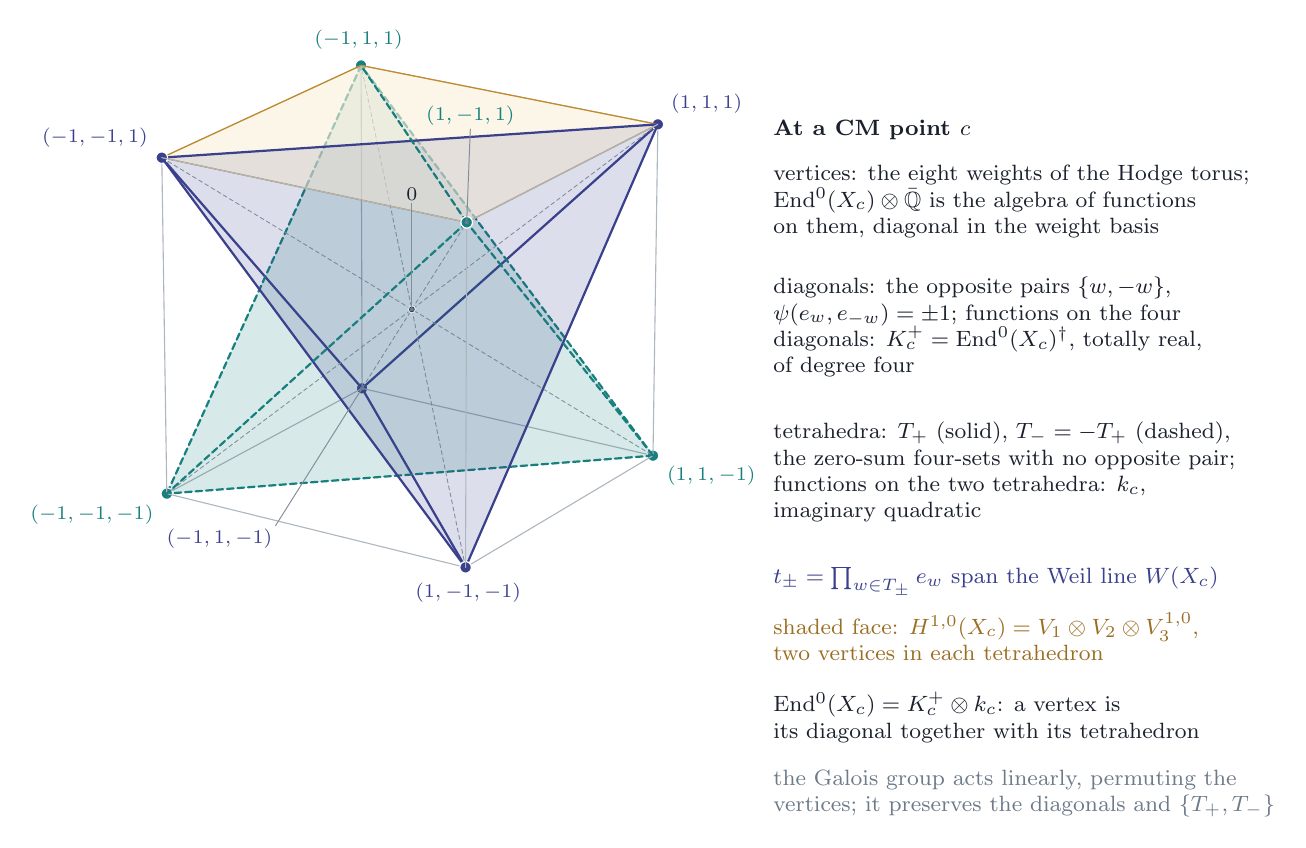
\begin{tikzpicture}[x=1cm,y=1cm,line join=round,line cap=round,
  font=\small,text=PInk,lbl/.style={inner sep=1pt}]
  \fill[PIndigo,draw=white,line width=0.45pt] (-0.6322,-1.0032) circle (2.10pt);
  \draw[PSlate!55,line width=0.4pt] (-0.6446,3.0973) -- (-0.6322,-1.0032);
  \draw[PSlate!55,line width=0.4pt] (3.0624,-1.8577) -- (-0.6322,-1.0032);
  \fill[PTeal,draw=white,line width=0.45pt] (-0.6446,3.0973) circle (2.10pt);
  \draw[PSlate!55,line width=0.4pt] (-0.6322,-1.0032) -- (-3.1121,-2.3403);
  \draw[PIndigo,line width=0.8pt] (3.1241,2.3494) -- (-0.6322,-1.0032);
  \draw[PTeal,line width=0.8pt,dash pattern=on 2.4pt off 1.4pt] (3.0624,-1.8577) -- (-0.6446,3.0973);
  \fill[PTeal,draw=white,line width=0.45pt] (3.0624,-1.8577) circle (2.10pt);
  \path[fill opacity=0.09,fill=PTeal,draw=none,line width=0.30pt] (3.0624,-1.8577) -- (-0.6446,3.0973) -- (-3.1121,-2.3403) -- cycle;
  \draw[PIndigo,line width=0.8pt] (-0.6322,-1.0032) -- (-3.1759,1.9265);
  \draw[PTeal,line width=0.8pt,dash pattern=on 2.4pt off 1.4pt] (-0.6446,3.0973) -- (-3.1121,-2.3403);
  \draw[PSlate!55,line width=0.4pt] (3.1241,2.3494) -- (-0.6446,3.0973);
  \draw[PIndigo,line width=0.8pt] (0.6820,-3.2769) -- (-0.6322,-1.0032);
  \draw[PTeal,line width=0.8pt,dash pattern=on 2.4pt off 1.4pt] (3.0624,-1.8577) -- (-3.1121,-2.3403);
  \path[fill opacity=0.09,fill=PIndigo,draw=none,line width=0.30pt] (3.1241,2.3494) -- (-0.6322,-1.0032) -- (-3.1759,1.9265) -- cycle;
  \draw[PSlate!55,line width=0.4pt] (3.1241,2.3494) -- (3.0624,-1.8577);
  \path[fill opacity=0.09,fill=PIndigo,draw=none,line width=0.30pt] (3.1241,2.3494) -- (0.6820,-3.2769) -- (-0.6322,-1.0032) -- cycle;
  \draw[PSlate!55,line width=0.4pt] (-0.6446,3.0973) -- (-3.1759,1.9265);
  \fill[PTeal,draw=white,line width=0.45pt] (-3.1121,-2.3403) circle (2.10pt);
  \path[fill opacity=0.09,fill=PIndigo,draw=none,line width=0.30pt] (0.6820,-3.2769) -- (-0.6322,-1.0032) -- (-3.1759,1.9265) -- cycle;
  \draw[PSlate!80,line width=0.32pt,dash pattern=on 1.5pt off 1.1pt] (3.1241,2.3494) -- (-3.1121,-2.3403);
  \draw[PSlate!80,line width=0.32pt,dash pattern=on 1.5pt off 1.1pt] (0.6820,-3.2769) -- (-0.6446,3.0973);
  \draw[PSlate!80,line width=0.32pt,dash pattern=on 1.5pt off 1.1pt] (-0.6322,-1.0032) -- (0.6964,1.1051);
  \draw[PSlate!80,line width=0.32pt,dash pattern=on 1.5pt off 1.1pt] (-3.1759,1.9265) -- (3.0624,-1.8577);
  \fill[PInk,draw=white,line width=0.45pt] (-0.0000,0.0000) circle (1.30pt);
  \path[fill opacity=0.09,fill=PTeal,draw=none,line width=0.30pt] (3.0624,-1.8577) -- (0.6964,1.1051) -- (-0.6446,3.0973) -- cycle;
  \fill[PIndigo,draw=white,line width=0.45pt] (3.1241,2.3494) circle (2.10pt);
  \draw[PSlate!55,line width=0.4pt] (3.0624,-1.8577) -- (0.6820,-3.2769);
  \path[fill opacity=0.09,fill=PTeal,draw=none,line width=0.30pt] (0.6964,1.1051) -- (-0.6446,3.0973) -- (-3.1121,-2.3403) -- cycle;
  \draw[PSlate!55,line width=0.4pt] (-3.1759,1.9265) -- (-3.1121,-2.3403);
  \path[fill opacity=0.09,fill=PTeal,draw=none,line width=0.30pt] (3.0624,-1.8577) -- (0.6964,1.1051) -- (-3.1121,-2.3403) -- cycle;
  \path[fill opacity=0.62,fill=WOchre,draw=POchre,line width=0.45pt] (3.1241,2.3494) -- (0.6964,1.1051) -- (-3.1759,1.9265) -- (-0.6446,3.0973) -- cycle;
  \draw[PIndigo,line width=0.8pt] (3.1241,2.3494) -- (-3.1759,1.9265);
  \draw[PTeal,line width=0.8pt,dash pattern=on 2.4pt off 1.4pt] (0.6964,1.1051) -- (-0.6446,3.0973);
  \draw[PSlate!55,line width=0.4pt] (0.6820,-3.2769) -- (-3.1121,-2.3403);
  \draw[PIndigo,line width=0.8pt] (3.1241,2.3494) -- (0.6820,-3.2769);
  \draw[PTeal,line width=0.8pt,dash pattern=on 2.4pt off 1.4pt] (3.0624,-1.8577) -- (0.6964,1.1051);
  \path[fill opacity=0.09,fill=PIndigo,draw=none,line width=0.30pt] (3.1241,2.3494) -- (0.6820,-3.2769) -- (-3.1759,1.9265) -- cycle;
  \fill[PIndigo,draw=white,line width=0.45pt] (-3.1759,1.9265) circle (2.10pt);
  \draw[PIndigo,line width=0.8pt] (0.6820,-3.2769) -- (-3.1759,1.9265);
  \draw[PTeal,line width=0.8pt,dash pattern=on 2.4pt off 1.4pt] (0.6964,1.1051) -- (-3.1121,-2.3403);
  \draw[PSlate!55,line width=0.4pt] (3.1241,2.3494) -- (0.6964,1.1051);
  \fill[PIndigo,draw=white,line width=0.45pt] (0.6820,-3.2769) circle (2.10pt);
  \draw[PSlate!55,line width=0.4pt] (0.6964,1.1051) -- (-3.1759,1.9265);
  \draw[PSlate!55,line width=0.4pt] (0.6964,1.1051) -- (0.6820,-3.2769);
  \fill[PTeal,draw=white,line width=0.45pt] (0.6964,1.1051) circle (2.10pt);
  \draw[PSlate!85,line width=0.35pt] (0.7423,2.2892) -- (0.6964,1.1051);
  \fill[PSlate] (0.6964,1.1051) circle (0.75pt);
  \draw[PSlate!85,line width=0.35pt] (-1.7305,-2.7460) -- (-0.6322,-1.0032);
  \fill[PSlate] (-0.6322,-1.0032) circle (0.75pt);
  \draw[PSlate!85,line width=0.35pt] (-0.0000,1.3450) -- (-0.0000,0.0000);
  \fill[PSlate] (-0.0000,0.0000) circle (0.75pt);
  \node[lbl,anchor=west,text=PIndigo,font=\scriptsize] at (3.2520,2.6107) {$(1,1,1)$};
  \node[lbl,anchor=west,text=PTeal,font=\scriptsize] at (3.1992,-2.1059) {$(1,1,-1)$};
  \node[lbl,anchor=south,text=PTeal,font=\scriptsize] at (0.7423,2.2892) {$(1,-1,1)$};
  \node[lbl,anchor=north,text=PIndigo,font=\scriptsize] at (0.7146,-3.4336) {$(1,-1,-1)$};
  \node[lbl,anchor=south,text=PTeal,font=\scriptsize] at (-0.6772,3.2540) {$(-1,1,1)$};
  \node[lbl,anchor=east,text=PIndigo,font=\scriptsize] at (-1.7305,-2.9112) {$(-1,1,-1)$};
  \node[lbl,anchor=east,text=PIndigo,font=\scriptsize] at (-3.3127,2.1747) {$(-1,-1,1)$};
  \node[lbl,anchor=east,text=PTeal,font=\scriptsize] at (-3.2400,-2.6017) {$(-1,-1,-1)$};
  \node[lbl,anchor=south,text=PInk,font=\scriptsize] at (-0.0000,1.3450) {$0$};
  \node[lbl,anchor=west,text=PInk,font=\footnotesize,align=left] at (4.5500,2.2829) {\textbf{At a CM point $c$}};
  \node[lbl,anchor=west,text=PInk,font=\footnotesize,align=left] at (4.5500,1.3690) {vertices: the eight weights of the Hodge torus;\\$\End^{0}(X_{c})\otimes\bar\QQ$ is the algebra of functions\\on them, diagonal in the weight basis};
  \node[lbl,anchor=west,text=PInk,font=\footnotesize,align=left] at (4.5500,-0.2258) {diagonals: the opposite pairs $\{w,-w\}$,\\$\psi(e_{w},e_{-w})=\pm1$; functions on the four\\diagonals: $K_{c}^{+}=\End^{0}(X_{c})^{\dagger}$, totally real,\\of degree four};
  \node[lbl,anchor=west,text=PInk,font=\footnotesize,align=left] at (4.5500,-2.0658) {tetrahedra: $T_{+}$ (solid), $T_{-}=-T_{+}$ (dashed),\\the zero-sum four-sets with no opposite pair;\\functions on the two tetrahedra: $k_{c}$,\\imaginary quadratic};
  \node[lbl,anchor=west,text=PIndigo,font=\footnotesize,align=left] at (4.5500,-3.4585) {$t_{\pm}=\prod_{w\in T_{\pm}}e_{w}$ span the Weil line $\HW(X_{c})$};
  \node[lbl,anchor=west,text=POchre!80!black,font=\footnotesize,align=left] at (4.5500,-4.1560) {shaded face: $H^{1,0}(X_{c})=V_{1}\otimes V_{2}\otimes V_{3}^{1,0}$,\\two vertices in each tetrahedron};
  \node[lbl,anchor=west,text=PInk,font=\footnotesize,align=left] at (4.5500,-5.1769) {$\End^{0}(X_{c})=K_{c}^{+}\otimes k_{c}$: a vertex is\\its diagonal together with its tetrahedron};
  \node[lbl,anchor=west,text=PSlate,font=\footnotesize,align=left] at (4.5500,-6.1519) {the Galois group acts linearly, permuting the\\vertices; it preserves the diagonals and $\{T_{+},T_{-}\}$};
\end{tikzpicture}
\end{document}
